\documentclass[11pt, letterpaper]{report}
\usepackage{geometry}
\usepackage{graphicx, subfigure,multirow, booktabs}
\usepackage[spanish]{babel}
\usepackage{xcolor}
\definecolor{darkblue}{rgb}{0, 0, 0.5}
\usepackage[colorlinks=true,linkcolor=black,anchorcolor=black,citecolor=darkblue,filecolor=black,menucolor=black,runcolor=black,urlcolor=darkblue]{hyperref}
\usepackage[utf8]{inputenc}
\usepackage[T1]{fontenc} 
\usepackage{setspace}
\geometry{lmargin=3cm, rmargin=3cm, tmargin=2.65cm, bmargin=3cm}
\usepackage[pages=some]{background}
\usepackage{natbib}
\usepackage{sectsty}
\usepackage{amssymb,amsmath}
\usepackage{blindtext}

\backgroundsetup{
	scale=1,
	angle=0,
	opacity=1,
	color=black,
	hshift=-159,
	contents={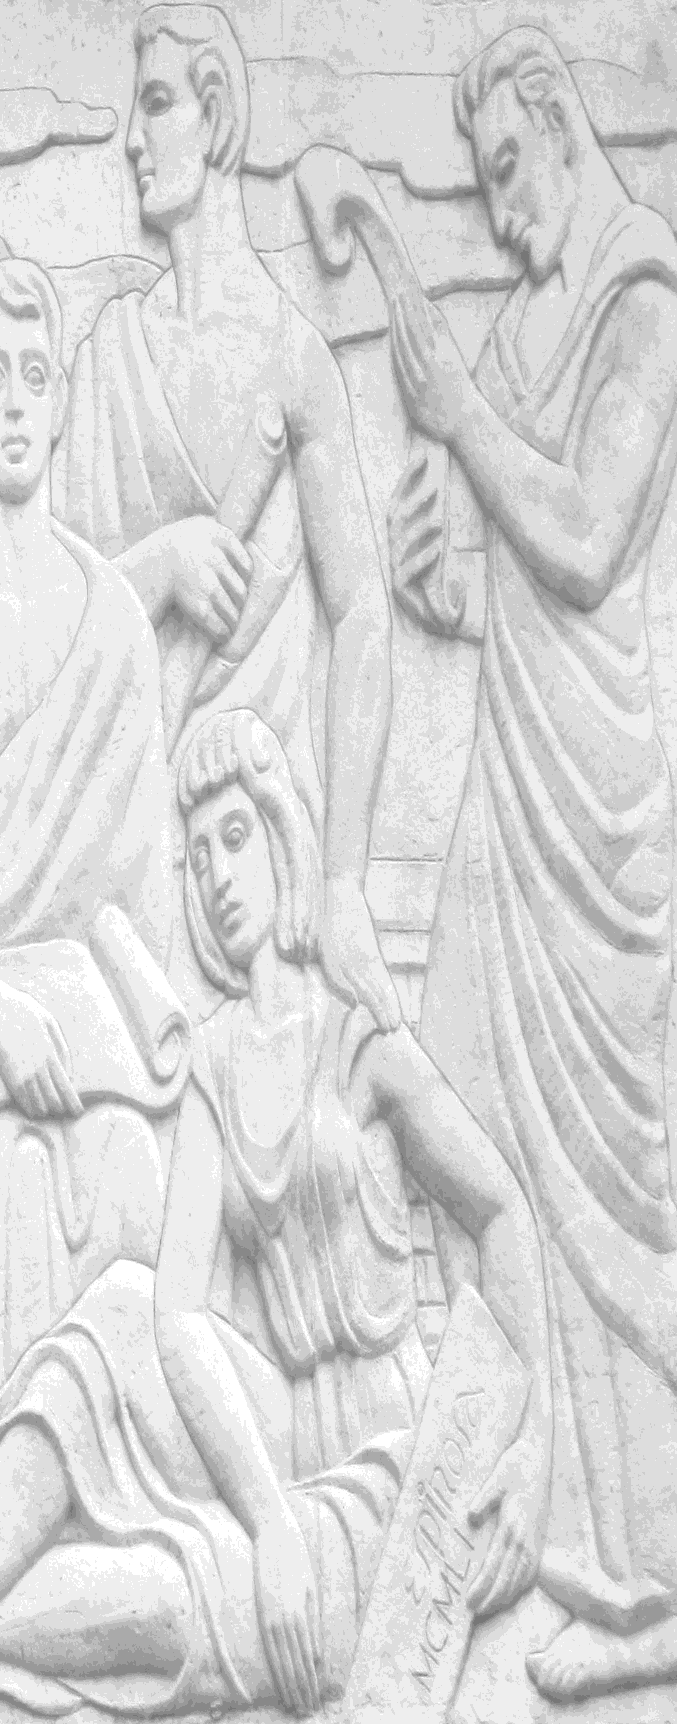
\includegraphics[width=0.48\paperwidth,height=\paperheight]{images/portada.png}}
}


\begin{document}
	\begin{titlepage}
	\begin{minipage}[t]{0.48\textwidth}
		\BgThispage
		\parbox{\textwidth}{}
	\end{minipage}
	\begin{minipage}[t]{0.55\textwidth}
			\parbox{\textwidth}{
				
\includegraphics[width=.8\textwidth]{images/logo.png}\\[0.5cm]
				\centering\textsc{Facultad de Ciencias Naturales y Exactas}\\[0.2cm]
				\centering\textsc{Departamento de Ciencia de la Computación}\\[2.2cm]
				\textbf{\LARGE Trabajo de Diploma en\\[-.1cm]Opción al Título de\\[-.1cm]Licenciado en Ciencia de la\\[-.1cm]Computación\\[2.2cm]}
				\Large  \textbf{Título}:\\
				\fontsize{18pt}{20pt}\selectfont Aprendizaje Profundo para el Perfilado de Usuarios en Redes Sociales\\
				\vspace{10mm}
				\begin{tabular}{rp{0.7\textwidth}}
					{\Large \bf Autor:} & {\Large Roberto Labadie Tamayo} \\[.5cm]
					{\Large \bf Tutores:} & {\Large Dr. Daniel Castro Castro} \\[.5cm]
					& {\Large M.Sc. Reynier Ortega Bueno} \\[.5cm]
				\end{tabular}
				
				\vspace{10mm}
				{\Large \textbf{Curso 2020-2021}}
			}
	\end{minipage}
	\end{titlepage}
	
	\pagenumbering{roman}
	\thispagestyle{empty} 	
	\chapterfont{\flushright}
	\renewcommand{\contentsname}{Contenido} \tableofcontents
	\renewcommand{\listfigurename}{Lista de Figuras} \listoffigures	
	\renewcommand{\listtablename}{Lista de Tablas} \listoftables
	\renewcommand{\tablename}{Tabla}
	\clearpage

	
	\pagenumbering{arabic}
\addcontentsline{toc}{chapter}{Introducción}
\chapter*{Introducción}
Internet se define como la interconexión mundial de redes individuales operadas por el gobierno, la industria, el mundo académico y las partes privadas. En cuestión de muy pocos años, Internet se consolidó como una plataforma muy poderosa que ha cambiado para siempre la forma de comunicarse.  Esta manera tan simple y accesible de compartir datos, ha propiciado un desplazamiento de los entes sociales hacia el uso casi exclusivo de este medio.
\\
Un rol fundamental dentro de este universo comunicativo lo juegan las redes sociales donde de acuerdo al sitio DataReportal\footnote{\url{https://datareportal.com/}} a finales de 2020 existían más de 3.8 mil millones de usuarios de los 4.5 mil millones de personas conectadas a Internet, lo cual implica un crecimiento desmedido de la cantidad de datos multimodales que se genera a diario.
\\
El mundo del Big Data \citep{Riahi2018BigDA} en el cual nos sumerge este hecho, reporta una situación beneficiosa para el desarrollo de procesos sociales, en cuanto a la cantidad de información brindada por los usuarios . 
Estos procesos van desde estudios de marketing donde la retroalimentación a partir de opiniones permiten dirigir de manera efectiva la promoción hacia grupos sociales específicos, hasta aplicaciones en el área de la Interacción Humano-Computadora (\textit{Human-Computer Interaction }HCI), donde el conocimiento de las características físicas y psicológicas de las personas permite personalizar la interfaz de comunicación. Sin embargo un cúmulo de información tan significativo, se hace imposible de tratar en un espacio de tiempo razonable a menos que se haga de manera automatizada.
\\
Diversos estudios se han dirigido al diseño de métodos para manejar tal cantidad de información y realizar inferencias a partir de la misma, a la vez que han contribuido al desarrollo en ramas tales como el Procesamiento del Lenguaje Natural (\textit{Natural Langauage Processing} NLP) y Visión por Computadoras (\textit{Computer Vision} CV) en el área de la Inteligencia Artificial (\textit{Artificial Intelligence} AI).
\\ 
Dentro del NLP, la tarea de Perfilado de Autores (\textit{Author Profiling AP}) \citep{Rosso2019,article} se encarga específicamente de realizar un análisis de la información textual elaborada por una persona que permita establecer atributos y patrones de comportamiento para caracterizarla en cuanto a sexo, rango de edades o rasgos personales (e.g si la persona es extrovertida o no, ideología política). Sin embargo, para el AP el hecho de que la información recuperada de estos textos varíe enormemente en términos de su formato aun cuando proviene de la misma persona, sumado a que las secuencias texuales constituyen información digital no estructurada, hacen desafiante el proceso de analizarla y clasificarla automáticamente. 
\\
Inicialmente este tipo de tareas se desarrollaban sobre contenido generado en textos formales, periódicos, cartas o revistas, sin embargo determinar el perfil de una persona mediante el análisis de su cuenta en una red social ha tomado un gran auge en los últimos años \citep{rangel:2018,rangel:2019,f6032ffbacb14369b7a45d1ba9bd0b8c}.
 Las redes sociales además de haber logrado acelerar la comunicación entre las personas así como reunir varias formas del pensamiento individual en un mismo espacio, se han convertido en un medio donde se desarrollan procesos negativos tales como, la divulgación de discursos de odio \citep{rangel2021profiling}, \textit{bullying} o de noticias falsas \citep{rangel:2020}. Este hecho introduce nuevos retos al AP con tareas que involucran la detección de elementos altamente subjetivas como la ofensa, la toxicidad en el lenguaje y otros patrones psicológicos de comunicación que hacen más complejo el perfilado en relación a otras tareas.  
\\
 La mayor parte de los avances en el desarrollo de sistemas de AP han sentado sus bases dentro del ambiente académico, reuniendo estudios tanto de la Ciencia de la Computación como de la Lingüística. Algunas de las campañas de evaluación más importantes donde se han compartido tareas de este tipo son \textit{Plagiarism, Authorship and Social Software Misuse} PAN\footnote{https://pan.webis.de/} y \textit{Evaluation of NLP and Speech Tools for Italian} EVALITA\footnote{http://www.evalita.it/}, los que se han dirigido últimamente al análisis del genero textual de micro-blogging  con un enfoque multilingüe, empleado en medios sociales como Twitter\footnote{https://twitter.com/}.
\\
Tradicionalmente se han empleado dos tipos de acercamientos que han probado empíricamente ser efectivos para tratar el AP en redes sociales: los \textit{basados en estilo}  y los \textit{basados en contenido}. Las propuestas basadas en estilo se refieren al hecho de analizar como los autores se expresan cuando escriben, en cambio la basada en contenido se apoyan en el área temática del texto analizado. La mayor contribución de varios trabajos se ha basado en la selección de atributos que permitan medir el estilo autor y el contenido simultáneamente mediante el empleo de métodos de Aprendizaje de Máquina (\textit{Machine Learning} ML).
\\
Un proceso crítico en este tipo de propuestas es la selección de rasgos para representar vectorialmente los elementos del texto,  en el cual pueden ser eliminados elementos que ayuden al modelo a discernir entre una clase u otra, en el caso de tareas de clasificación, pero también se puede introducir información ruidosa y de igual forma afectar su desempeño. 
\\
\\
En los últimos años dentro del Machine Learning ha tenido un auge enorme el Aprendizaje Profundo (\textit{Deep Learning} DL) en las áreas de CV y NLP, estableciendo nuevos estados del arte en la mayoría de sus tareas \citep{electronics8030292}. Este auge estuvo condicionado por las capacidades de procesamiento de las nuevas computadoras y la cantidad de datos disponibles. Los modelos de DL han mostrado una gran habilidad para aprender representaciones de rasgos (\textit{features}) con un alto nivel de abstracción. Estas representaciones capturan elementos que son posiblemente omitidos mediante la extracción manual de features y que facilitan el proceso de inferencia de los propios modelos de DL y de los métodos más tradicionales de ML. 
\\
Dentro del AP también se ha introducido el Aprendizaje Profundo con resultados alentadores. Sin embargo la mayoría de los modelos alcanzan mejores resultados al analizar la tarea a la que se orienta el perfilado cuando se emplean para clasificar mensajes individuales en lugar del perfil completo, e.g., se desempeñan mejor en la tarea de detección de odio en un tweet que en la detección de un perfil que tiende a usar un discurso de odio. 
\\
Por otro lado, las necesidades que cubren las tareas de AP incluyen la no sensibilidad de los sistemas ante la variación del idioma en el que la persona postee un mensaje o escriba una carta, es por ello que urge la extensión de los modelos de AI propuestos al esquema multilingüe que predomina en redes sociales como Twitter. \\Este trabajo de tesis se enmarca en el perfilado de autores en redes sociales empleando técnicas de Aprendizaje Profundo para el modelado y la clasificación de los perfiles teniendo en cuenta el enfoque multilingüe propio de este medio. 

\addcontentsline{toc}{section}{Problemática}
\section*{Problemática}
La mayoría de los trabajos existentes que emplean DL para resolver tareas de perfilado de autores en redes sociales, tanto tradicionales (e.g., determinar rango de edades, sexo, etc.) como las más recientes (e.g. detección de divulgadores de discursos de odio en redes sociales o noticias falsas) ven afectado su desempeño al tratar con las secuencias muy largas que se pueden generar al analizar un perfil completo a la vez, en vez de mensaje a mensaje. La perdida de información (\textit{information vanishing}) en este tipo de secuencias en términos de relaciones a largo plazo que presentan las estructuras sintácticas del lenguaje, es la causa fundamental de esta dificultad. Por esta razón sería conveniente dividir el problema de ``clasificar un perfil'' en subproblemas y construir una arquitectura modular, en la que primero se modele el perfil y luego este sea clasificado.
\\
Por otro lado en Cuba existe un limitado tratamiento y aplicación de este tipo de métodos automatizados para llevar acabo tareas de impacto como las mencionadas, ya sea en el área forense o empresarial .

\addcontentsline{toc}{section}{Hipótesis}
\section*{Hipótesis}
Dividir el proceso de clasificación de un perfil dentro de una tarea en: (1) codificar los mensajes individualmente y (2) modelar-clasificar el perfil, puede ayudar a prevenir la perdida de información generada del análisis de largas secuencias. Esto sumado a la capacidad de representar la información no estructurada de los métodos de DL puede influir positivamente en la precisión de las predicciones.  Además, proponer un modelo lo suficientemente robusto, podría incentivar el empleo de esos métodos automatizados  de AP en nuestro país.

\addcontentsline{toc}{section}{Objetivos}
\section*{Objetivos}
\subsection*{Objetivo General}
Diseñar una arquitectura de Aprendizaje Profundo modular para resolver la tarea de Perfilado de Autores en redes sociales teniendo en cuenta un enfoque multilingüe.
\subsection*{Objetivos Específicos}
\begin{enumerate}
	\item Diseñar una arquitectura que capture rasgos abstractos que permitan clasificar un perfil de usuario de una red social atendiendo tanto a tareas relacionadas con características demográficas de los autores, como con aspectos psicológicos de los mismos.
	\item Extender la arquitectura propuesta a un enfoque multilingüe de las tareas evaluadas.
	\item Evaluar y analizar el empleo de arquitecturas modulares basadas en DL sobre colecciones de datos propuestas en tareas de AP compartidas en la plataforma PAN (2019, 2020, 2021).
\end{enumerate}
\section*{Estructura del Trabajo}
Este trabajo esta estructurado en tres capítulos además del introductorio y una última sección en la que se describen las conclusiones de las modelaciones y se proponen  caminos a seguir para trabajos futuros. Cada uno de los capítulos se listan a continuación: 

%%Poner la reerencia de cada capitulo cuando este listo
\begin{itemize}
	\item En el Capítulo 1 se describen de manera breve métodos del estado del arte así como conceptos básicos relacionados con el Machine Learning necesarios para la comprensión de este trabajo.
	\item El Capítulo 2 describe las tareas de AP en las que se evaluarán las arquitecturas propuestas, así como los datos anotados sobre los cuales se basan los procesos de entrenamiento y evaluación.
	\item En el Capítulo 3 se exponen los experimentos realizados en el proceso de ajuste de cada unos de los modelos y sus módulos sobre los lenguajes estudiados. 
\end{itemize}
. 
	
\chapter{Fundamentos}

\section{Estado del Arte}\label{SOTA}

El Procesamiento del Lenguaje Natural, como cualquier tarea llevada a cabo por un algoritmo de Machine Learning, se basa en el análisis de un conjunto de rasgos del objeto a procesar, con la finalidad de realizar inferencias que permitan al sistema computarizado interactuar con el usuario.
\\
Para la tarea de  AP no es diferente, por lo que la mayoría de los trabajos se dirigen al desarrollo de una efectiva selección de rasgos, estableciéndose dos categorías fundamentales; los rasgos de estilo y los de contenido.  
\\
El análisis de estilo se enfoca en la detección de rasgos estilísticos del autor que sean lo suficientemente invariantes a lo largo de los pasajes escritos, pero que varíen de un autor a otro. Ejemplos de estos podrían ser la longitud media de las oraciones o la cantidad esperada de símbolos de puntuación, emoticones, preposiciones o  adverbios en un párrafo.
\\
Por otra parte el análisis de contenido se enfoca en la información contextual siguiendo la misma estrategia del análisis de estilo, i.e., llevar información estadística de la presencia de determinado conjunto de palabras o estructuras gramaticales. Este tipo de rasgos incluye el uso de n-gramas de palabras y caracteres, \textit{slang words}\footnote{ \textit{slang} se refiere a un lenguaje muy informal empleado por un grupo particular de personas.}, Bolsas de Palabras (\textit{Bag of Words} BoW) \citep{DBLP:conf/clef/Pizarro19,DBLP:conf/clef/Valencia-Valencia19}, palabras concluyentes (e.g., finalmente, para concluir, en conclusión, etc.)  y lexicones de palabras.
Dentro de este último método para categorizar palabras, el más empleado es el sistema \textit{Linguistic Inquiry and WordCount LIWC} \citep{pennebaker2015development} el cual contiene alrededor de 70 diccionarios de lexicones divididos en categorías como; Preocupaciones personales (\textit{Personal Concerns}), Discurso informal (\textit{Informal Speech}), Impulsos (\textit{Drives}) y necesidades fundamentales (\textit{Basics Needs}), etc.
\\\\
Estos dos grupos de rasgos, de estilo y contenido, son ortogonales puesto que los rasgos que se tienen en cuenta para capturar estilo, son precisamente aquellos que son independientes del tópico, por lo cual se ha hecho habitual el uso de enfoques que los combinen a ambos. Por otro lado el empleo de elementos contextuales implica introducir en el proceso de clasificación un sesgo hacia una clase que este más representada por determinado tema, e.g., según \citep{schler2006effects} estos rasgos pueden facilitar la determinación del sexo del autor ya que por ejemplo los hombres mayormente tienden a hablar de política y noticias, mientras que las mujeres se muestran más interesadas por la moda, fiestas y prendas de vestir; sin embargo es posible encontrar una mujer que regularmente postee tweets relacionados con deportes o automóviles, luego este perfil sería potencialmente mal clasificado por un modelo de AP basado en rasgos de contenido.
\\
La mayoría de los trabajos de Machine Learning han usado métodos de clasificación tradicionales como Regresión Logística (Logistic Regression LR) \citep{DBLP:conf/clef/Valencia-Valencia19}, Máquina de Vectores de Soporte (\textit{Support Vector Machines} SVM) \citep{DBLP:conf/clef/Pizarro19}  y Bosques Aleatorios (\textit{Random Forest} RF) \citep{DBLP:conf/clef/Johansson19} combinando conjuntos de rasgos que responden a estas clasificaciones.
\\
\\
 Con la introducción del Deep Learning en el NLP esta tendencia a la extracción manual de rasgos de tipo estadístico ha sido desplazada por el aprendizaje de rasgos abstractos que representan a las estructuras gramaticales atendiendo no solamente a su significado semántico como elementos aislados del texto, sino que además tienen en cuenta el contexto en el que son empleados, facilitando la comprensión y clasificación de los textos tanto a los propios modelos de DL como a los tradicionales de ML. Este tipo de enfoques se basan fundamentalmente en el uso de \textit{embeddings} preentrenados con distintas estrategias \citep{DBLP:conf/clef/JooH19,DBLP:conf/clef/Lopez-Santillan19}, principalmente Word2Vec \citep{DBLP:conf/nips/MikolovSCCD13}, Glove\citep{pennington2014glove} y Fasttext\citep{bojanowski2016enriching}.
 \\
 Las Redes Neuronales Artificiales como mecanismos de aprendizaje y clasificación, por su parte han logrado un desempeño superior a los métodos tradicionales de ML en muchas tareas de NLP, teniendo en cuenta que aprenden a decidir que elemento del texto tomar como rasgo significativo a la hora de modelar los objetos. Esquemas especializados en análisis de secuencias, como las Redes Neuronales Recurrentes (RNN) \citep{DBLP:conf/clef/DiasP19,bakhteev:2020} y las arquitecturas \textit{Transformers} (Transformadoras) \citep{iyer:2020,baruah:2020} se han empleado satisfactoriamente para el perfilado de autores en los últimos años, pero también se ha extendido el uso de arquitecturas diseñadas inicialmente para el tratamiento de otro tipo de información estructurada como las imágenes, tal es el caso de las Redes Neuronales Convolucionales (CNN) \citep{DBLP:conf/clef/PetrikC19,DBLP:conf/clef/Lopez-Santillan19}.
 \\
 \\
 En los últimos años dentro de PAN se han propuesto tareas de perfilado que van desde la predicción de sexo y variedad del idioma  hasta la detección de perfiles manejados por bots y perfiles que tienden a difundir discursos de odio en el medio social. En la mayoría de estas tareas los trabajos con un mejor desempeño se han enmarcado en técnicas tradicionales de ML, tal es el caso de \citep{basile:2017} en la tarea \textit{Gender and Language Variety Identification in Twitter at} PAN 2017, quienes emplearon rasgos construidos a partir de una medida no estándar de frecuencia de términos sobre unigramas de palabras y n-gramas de caracteres para entrenar una SVM y \citep{martinc:2017}  que combinaron n-gramas de palabras, caracteres y Elementos del Discurso (\textit{Part of Speech} POS), además de información de sentimientos relacionada con el uso de emojis y conteo de elongación de caracteres, con otros rasgos de estilo para modelar el perfil y entrenar un Regresor Logístico. 
 \\
 La tarea \textit{Bots and Gender Profiling in Twitter at} PAN 2019\footnote{\url{https://pan.webis.de/clef19/pan19-web/author-profiling.html}} consistente en determinar si una cuenta de Twitter pertenece a un bot o a un humano y en el segundo caso, inferir el sexo; \citep{DBLP:conf/clef/Pizarro19} obtuvo la mejor precisión con una SVM, combinando representaciones de los tweets mediante \textit{tf-idf} de n-gramas de palabras y caracteres. De igual forma \citep{DBLP:conf/clef/Johansson19} trató de dar solución a la tarea empleando ML con Random Forest y rasgos de estilo como longitud de los tweets, número de letras mayúsculas, URLs, menciones, cantidad de RTs, así como rasgos de contenido, específicamente ocurrencia de términos y etiquetas de POS.
 \\ 
 Nuevamente en PAN 2020, en la tarea \textit{Profiling Fake News Spreaders on Twitter}\footnote{\url{https://pan.webis.de/clef20/pan20-web/author-profiling.html}}, para detectar divulgadores de noticias falsas, \citep{pizarro:2020} se basó en la combinación de vectores de \textit{tf-idf} de n-gramas de palabras y caracteres para representar los tweets y clasificar los perfiles con una SVM. Mientras el modelo propuesto por \citep{buda:2020} consistió en un Regresor Logístico que combina las predicciones de cinco submodelos: (i) n-gramas con Regresor Logístico,(ii) n-gramas con SVM, (iii) n-gramas con Random Forest, (iv) n-gramas con XGBoost y (v) XGBoost con features de estilo.
 \\
Diversos modelos de DL empleando las arquitecturas citadas anteriormente (e.g., RNN y CNN) han sido propuestos a lo largo de estas competiciones, aunque ninguno de ellos mostró una precisión superior a la de los métodos tradicionales de ML. Sin embargo, en la tarea \textit{Profiling Hate Speech Spreaders on Twitter at} PAN 2021 \footnote{\url{https://pan.webis.de/clef21/pan21-web/author-profiling.html}}, consistente en determinar cuando un perfil era divulgador de contenido relacionado con el odio a grupos sociales específicos, el modelo con mejor desempeño, propuesto por \citep{sinno:2021} empleó una Red Neuronal Convolucional sobre la representación de los perfiles con \textit{embeddings} de palabras. 
\\\\
Uno de los mayores problemas con los enfoques predominantes es que los rasgos extraídos son muy dependientes del contexto lo cual puede crear una alta sensibilidad de los modelos ante datos que no correspondan a los corpus con los que han sido refinados sus parámetros o como ya hemos expuesto tengan un sesgo hacia alguna clase. Por ejemplo \citep{Newman2008GenderDI} expone que las mujeres tienden a usar emoticones con mayor regularidad que los hombres, lo contrario de lo concluido por \citep{Schwartz2013PersonalityGA}. Esto nos sugiere que métodos tan rigurosamente refinados como lo son los dependientes de rasgos manualmente extraídos tienen una menor robustez ante arquitecturas \textit{End-to-End} como las de Deep Learing.

\section{Marco Teórico}

En este epígrafe se realiza un acercamiento hacia los temas y arquitecturas de Machine Learning necesarios para la comprensión de los modelos propuestos en el trabajo.

\subsection{LSTM: Long Short-Term Memory Neural Networks}

	Las LSTM son un tipo de Redes Neuronales Recurrentes, las cuales están especializadas en el análisis de datos secuenciales. 
	Las RNNs tienen una unidad principal (la unidad recurrente) la cual explora la secuencia de datos de entrada de un elemento a la vez, ya sea de izquierda a derecha o viceversa. Al analizar un elemento para determinar su estado oculto, se comparte la información capturada en pasos anteriores del recorriendo. Esto es, sea $h_{t-1}$ el último estado oculto computado, $x_t \in \Re^d$ el $t-esimo$ elemento de la secuencia de entrada y $f$ una función de no linealidad. El estado oculto actual, se define como:
	\begin{equation}
		h_t = f(W_xx_t + W_hh_{t-1} + b_h)
		\label{rrn_form}
	\end{equation}
	Donde $W_x \in Re^{n_u\times d}$ y $W_h \in Re^{n_u\times n_u}$ son matrices de parámetros y $b_h \in R^{n_u}$ el término de sesgo (\textit{bias}), con $n_u$ el número de neuronas y $d$ la dimensión de los vectores que representan a los elementos de la secuencia.
	De esta forma la arquitectura aprende a considerar la información que tiene determinada influencia sobre el elemento de la secuencia que se analiza en cada paso como se muestra en la \figurename~\ref{rnn}, lo que le otorga una especie de ``memoria''.
	\begin{figure}[!thb]
		\begin{center}
			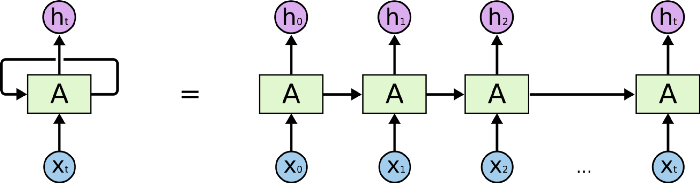
\includegraphics[width=250pt]{images/rnn.png}
		\end{center}
		\caption[Red Neuronal Recurrente]{Red Neuronal Recurrente sobre la secuencia $X_t$. \citep{agarwala2017music}}
		\label{rnn}
	\end{figure}
	\\
	Sin embargo, debido a que en las RNNs durante el proceso de \textit{backpropagation}, en el que se ajustan los parámetros de la red, cada neurona en la unidad principal calcula su gradiente para un paso del recorrido de la secuencia con respecto a su estado en el paso posterior, mediante la ley de la cadena, ocurre un decrecimiento exponencial de los valores de las derivadas parciales conocido como \textit{gradient vanishing}, lo que hace que los parámetros a penas se actualicen y se dificulte el aprendizaje de relaciones a largo plazo, de aquí su ``Short-Term Memory''.
	\\
	Esta limitación es lo que las LSTM tratan de solucionar introduciendo compuertas que deciden que información preservar u ``olvidar'' de los estados previos en el recorrido por la secuencia de la siguiente forma:
	\\
	Sean $W_f, W_i, W_o \in \Re^{n_u\times d}$ y $U_f, U_i, U_o \in \Re^{n_u\times n_u}$ las matrices de parámetros de la compuerta de ``olvidar '', entrada y salida respectivamente y $b_f, b_i, b_o \in \Re^{n_u}$ sus respectivos términos de bias:
	
	\begin{equation}
		\begin{split}
		i_{t} &= \sigma(W_i x_t + U_i  h_{t-1} + b_i)\\
		o_{t} &= \sigma(W_o x_t + U_o h_{t-1} + b_o)\\
		f_t &= \sigma(W_{f} x_t + U_f   h_{t-1} + b_f) 
		\end{split}
		\label{lstm_gates}
	\end{equation}
	\\
	Una codificación potencial $\hat{c}_t$ considerando el elemento $x_t$ de la secuencia y el estado previo $h_{t-1}$ esta dado por:
	\begin{equation}
		\hat{c}_{t} = \sigma(W_cx_t + U_c h_{t-1} + b_c)
		\label{lstm_pu}
	\end{equation}
	\\
	Donde $W_c\in\Re^{n_u\times d}$, $U_c\in\Re^{n_u\times n_u}$ y  $b_c\in\Re^{n_u}$. Luego la codificación $x_t$ teniendo en cuenta la codificación del elemento anterior y $h_t$ quedan definidos por:
	 \begin{equation}
	 	\begin{split}
	 		c_{t} &= f_tc_{t-1} +i_t\tanh(\hat{c}_{t})\\
	 		h_t &= o_t\tanh(c_t)
	 	\end{split}
	 	\label{lstm_hstate}
	 \end{equation}
 
 
\subsection{Redes Neuronales Convolucionales sobre secuencias}
	
	La arquitectura de una CNN \citep{lecun1998gradient} sobre una secuencia de texto es capaz de capturar dependencias temporales a corto plazo mediante filtros unidimensional que analizan n-gramas de palabras o caracteres y cuyos parámetros son compartidos durante cada paso de manera similar a las LSTM.
	\\
	Esto es, sea $X \in \Re^{l\times d}$ la secuencia de entrada de longitud $l$ donde cada elemento es un vector $d-dimensional$, $F_k$ el conjunto de filtros con ventana $k$ de una capa convolucional, cada uno de los ${F_k}_i \in \Re^{k\times d}$ son inicializados de manera independiente y de la misma forma aprenden a capturar relaciones a corto plazo  dentro en $X$. La operación convolución (\textit{conv-op}) transforma a $X$ en una nueva secuencia $X' \in \Re^{(l - k) \times n_f}$ donde $n_f = |F_k|$ de la siguiente forma:
	
	\begin{equation}
		X'_{ij} = \sum X_{[i:i+k]} * {F_k}_j ~~~ para ~~~ j \in [0, F_k-1], \;i \in [0, l-k]
	\end{equation}
	\\
	Como se puede observar en la \figurename~\ref{cnn} donde se representa un paso del desplazamiento de la ventana de uno de los filtro:
	\begin{figure}[!thb]
		\begin{center}
			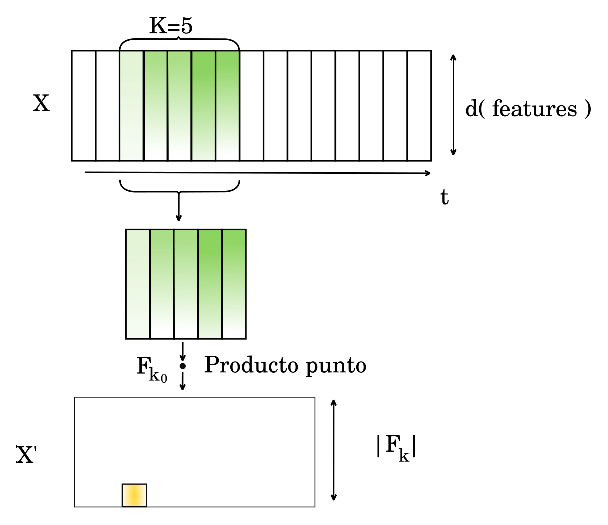
\includegraphics[width=250pt]{images/cnn.eps}
		\end{center}
		\caption[Operación Convolución. CNN]{Operación convolución sobre $X$ con filtros de tamaño de ventana k. }
		\label{cnn}
	\end{figure}
	\\
	Vinculada a la \textit{conv-op} en este tipo de arquitectura se suele emplear además una capa de \textit{pooling}, en la cual se combinan los valores de elementos en una vecindad para hacer que la red aprenda de manera más rápida a determinar los rasgos más importantes mediante la reducción de la dimensionalidad de la secuencia ya sea seleccionando los valores mas altos de las activaciones o su valor esperado en dicha vecindad. Esta operación de \textit{pooling} con una ventana de tamaño $k$  sobre una secuencia $X$ esta definida por:
	\begin{equation}
		X'_i = f(X_{[i:i+k]}) ~~ para ~~~  \;i \in [0, l-k]
	\end{equation}
	\\
	Donde $f$ es la función de \textit{pooling}, regularmente empleadas las funciones $Max$ o $Avg$.
		
\subsection{Mecanismos de Atención}\label{atencion}

	Los mecanismos de atención, son técnicas de procesamiento de las entradas de una arquitectura o de algún resultado intermedio que permiten a la red prestar más ``atención'' a elementos específicos de una secuencia o establecer la importancia relativa sobre un elemento del resto. En la práctica, la atención permite a las redes neuronales aproximarse al mecanismo de atención visual que utilizan los humanos.

	\subsubsection{Self-Attention}
	
		Sea $x_t$ la representación del $t-esimo$ elemento de la secuencia, una capa de \textit{self-attention} (auto-atención), captura en una matriz $A$ cuan similar es $x_t$ con sus vecinos. Específicamente $\alpha_{t, t'} \in A$ expresa la relación de $x_t$ con $x_t'$ y de manera similar al de una red recurrente, este valor se calcula como:
		\begin{equation}
			\begin{split}
				g_{t, t'} &= \tanh(W_{x}x_t + W_{x{t'}}x_{t'} + b_g)\\
				a_{t, t'} &= \sigma({W_{a}g_{t, t'} + b_{a}}) 
			\end{split}
		\end{equation}
		\\
		Donde $\sigma$ es la función sigmoide, $W_{x}, W_{x{t'}} \in \Re^{n_u \times d} $ son las matrices de parámetros encargadas de codificar la información de $x \text{ y } x'$ para expresar su compatibilidad, $W_a \in \Re^{n_u \times n_u}$ la matriz de parámetros correspondiente a su combinación no lineal y $b_g \text{ y } b_a$ los correspondientes términos de bias.
		\\
		A partir de $A$ el estado correspondiente al vector $x_t$, $\hat{x}_t$ está dado por la suma ponderada de sus elementos vecinos $x'_t$:
		
		\begin{equation} \label{attention}
			\hat{x}_t = \sum \limits_{i=0} a_{t,t'}x_{t'}
		\end{equation}
		\\
		Luego $\hat{x}_t$ expresa cuan atendido debe ser $x_t$ condicionado por el contexto de su vecindad.
	
	\subsubsection{Scaled Dot-Product Attention}
		
		El mecanismo \textit{Scaled Dot-Product Attention} (Atención con Producto-Punto Escalado) primero mapea cada elemento de la secuencia con tres representaciones (\textit{query} y un par \textit{key-value}) para calcular el índice de compatibilidad entre cada par de elementos. Luego, para cada $x_t$ es evaluada su compatibilidad con respecto a cada uno de los  elementos vecinos; relacionando su \textit{query} ($q_t$) con las \textit{keys} de los vecinos ($k_{t'}$), estos valores de compatibilidad son escalados y normalizados con la función $softmax$ y empleados para ponderar los vectores de \textit{value} ($v_t$). Finalmente la representación de $\hat{x}_t$ es calculada como la suma ponderada de los $v_t$. En forma matricial queda expresado como:
		
		\begin{equation}
			Attention(Q, V, K) = softmax(\frac{Q\times K^T}{\sqrt{d_k}})\times V
			\label{dotP-att}
		\end{equation} \\
		Donde $Q, K \in \Re^{n\times d_k} \text{ y } V \in \Re^{n\times d_v} $ son el resultado del producto de las matrices de parámetros de \textit{query}, \textit{key} y \textit{value} con los elementos de la secuencia respectivamente, por tanto en la fila $t$ contienen el mapeo del elemento $x_t$ y  $d_k,d_v$ corresponden a la dimensionalidad de las vectores de \textit{key} y \textit{value} respectivamente.
		
\subsection{Transformers}

	La arquitectura Transformer (\figurename~\ref{transformer}), basada en mecanismos de atención, específicamente \textit{multihead attention} \citep{vaswani2017attention}, está diseñada para tratar problemas de \textit{machine translation} y la conforman dos módulos, el primero conocido como \textit{Encoder} (Codificador) es alimentado con una secuencia textual y se encarga de encontrar una codificación para cada elemento teniendo en cuenta la información de su contexto. El segundo módulo, \textit{Decoder} produce los elementos de una nueva secuencia en el modelado de lenguaje, haciéndolo de uno a la vez, teniendo en cuenta los elementos generados anteriormente y las codificaciones obtenidas por el Encoder de la secuencia de entrada.
	\\
	La principal ventaja de las Transformers con respecto a las arquitecturas secuenciales más tradicionales, e.g., GRU y LSTM es que en vez de analizar la información textual en una dirección, esta toma en consideración la entrada completa relacionando cada elemento con el contexto de su vecindad simultáneamente lo cual evita el problema de ``memoria'' a corto plazo de las RNN.  Sin embargo, pudiera parecer que existe una pérdida de la percepción del tiempo al analizarlo todo a la vez, es por esto que además de representar el texto con un \textit{embedding} de palabras, se tiene en cuenta un \textit{encoding} de posición. 
	\begin{figure}[!thb]
		\begin{center}
			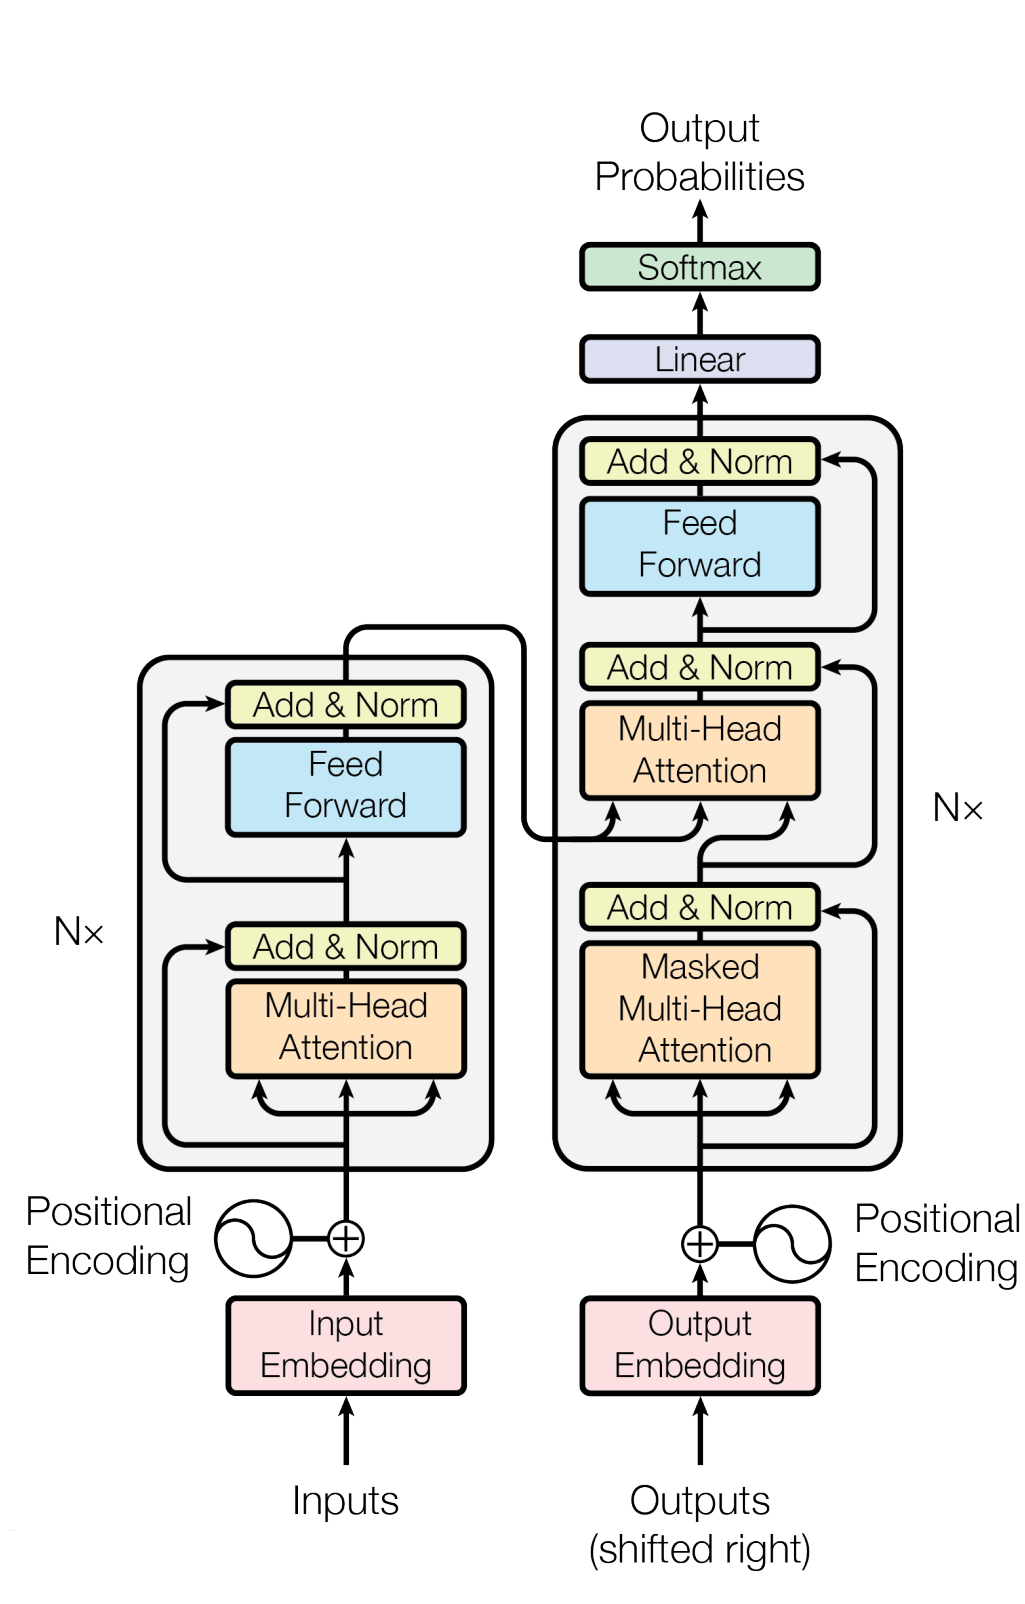
\includegraphics[width=.5\linewidth, height=.5\textheight]{images/transformer.png}
		\end{center}
		\caption[Arquitectura Transformer]{Arquitectura Transformer. Módulo Izquierdo, Codificador. Módulo Derecho, Decodificador. \citep{vaswani2017attention} }
		\label{transformer}
	\end{figure}
	\\
	En la \figurename~\ref{transformer} se observan cada uno de los módulos los cuales se apilan ($N_x$), i.e., antes de que el Decoder reciba la información codificada de la secuencia de entrada, esta transita por una serie de bloques codificadores haciendo uso de una red residual para prevenir cualquier pérdida de la información.
	\\
	Dentro de la mayoría de las tareas de NLP este tipo de modelo ha alcanzado nuevos estados del arte simplemente haciendo \textit{transfer learning} del modulo de Encoder hacia la tarea específica. Este módulo es entrenado en dos tareas: (i) predecir palabras enmascaradas de la secuencia de entrada; (ii) dadas dos oraciones, predecir si una está a continuación de la otra en el texto, lo cual hace que el modelo llegue a ``entender'' el funcionamiento del lenguaje y sea relativamente fácil de entrenar sobre otras tareas como el análisis de sentimientos. Para la tarea de predicción de la próxima oración (\textit{Next Sentence Prediction} NSP), dado el par de oraciones como una secuencia, se añade un \textit{token} [CLS] al inicio del cual se toma su estado oculto para realizar la clasificación y otro [SEP] al final de cada oración. 
	
\subsection{Redes Neuronales Convolucionales en Grafos}
	
	La principal diferencia entre las CNNs y las Redes Neuronales Convolucionales en Grafos (\textit{Graph Convolutional Neural Nets }GNN) es que las primeras están diseñadas especialmente para tratar datos regularmente estructurados (Euclideanos), mientras que las GNN son su versión generalizada capaz de extraer información en datos donde no existe una relación de orden entre un nodo y otro y las conexiones entre cada uno de ellos es variable (datos irregulares o datos estructurados no Euclideanos), estas dos propiedades son totalmente opuestas a las relaciones que existen entre los píxeles de una imagen (\figurename~\ref{euclidian-non}).
	\begin{figure}[!thb]
		\centering
		\subfigure[Datos Estructurados Euclideanos]{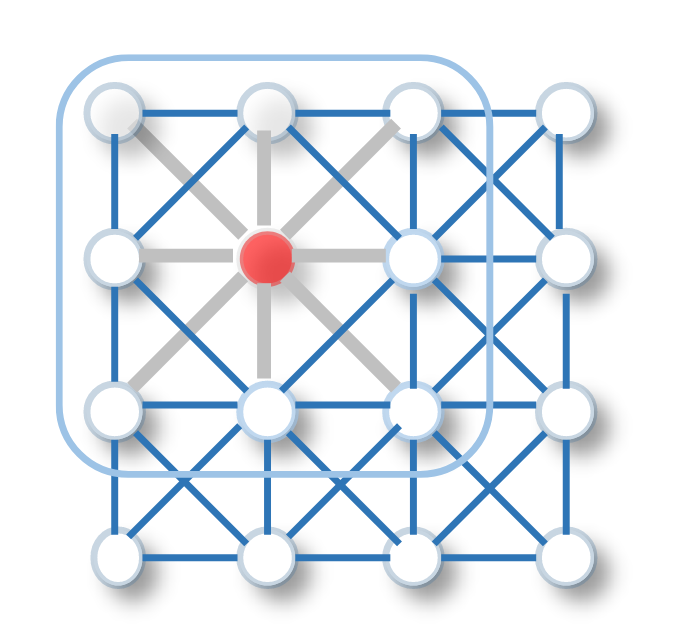
\includegraphics[width=0.35\textwidth]{images/cnn-gnn.png}} \hspace{10mm}
		\subfigure[Datos con Estructura No Euclideana]{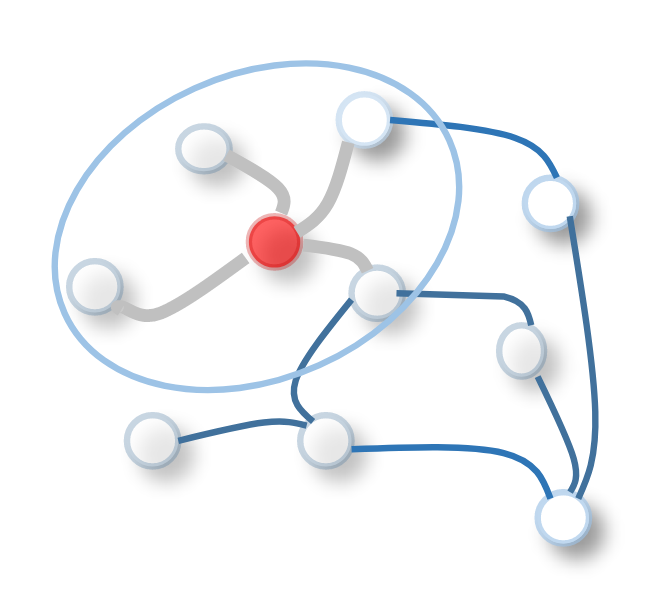
\includegraphics[width=0.35\textwidth]{images/gnn-gnn.png}} 
		\caption[Relación de Estructura en los Datos]{Relación de Estructura en los Datos. \citep{Wu_2021}}
		\label{euclidian-non}
	\end{figure}
	\\
	Un uso típico de las GNN es la clasificación de nodos en una estructura. En este tipo de problema el nodo $v$ se caracteriza por un conjunto de features $x_v$ y corresponde a una clase $t_v$. Dado un grafo $G = (V, E)$ parcialmente etiquetado, nuestro objetivo es predecir a que clase corresponde cada nodo no etiquetado. Mediante una GNN, cada nodo comparte información con su vecindad y transforma su representación a un estado $h_v$ de manera que exprese como este pertenece a su contexto. Específicamente,	
	\begin{equation}
		h_v = f(x_v, E_v, H_v, X_v)
	\end{equation}
	\\
	Donde $E_v = \{(i, j)| (i, j) \in E, v \in \{i, j\}\}$,  $H_v = \{h_u| u \in \mathcal{N}(v)\}$ con $\mathcal{N}(v)$ el conjunto de nodos de la vecindad de v y $X_v = \{x_u| u \in \mathcal{N}(v)\}$. Dentro del espacio imagen de $f$ es de nuestro interés que cada nodo tenga un estado $h_v$ unívoco, por lo que apoyándose en el teorema del punto fijo \citep{brown1988fixed} es posible encontrar en un proceso iterativo de actualizaciones con determinados parámetros para nuestra función $f$ este $h_v$ contextualizado. El proceso de actualizaciones llevado a cabo dado una función $f$, es conocido como paso de mensajes. Luego, en forma matricial el estado de todos los nodos en la actualización $t+1$ esta dado por:
	
	\begin{equation}
		H^{t+1} = F(H^t, X)
	\end{equation} 
	\\
	Con $H$ y $X$ matrices donde a cada fila $i$ le corresponde $h_i \text{ y } x_i$ respectivamente. Luego, la clasificación de un nodo es llevada a cabo mediante la una nueva función $g$:	
	
	\begin{equation}
		t_v = g(h_v, x_v)
	\end{equation}
	\\
	Muchos diseños de la función de agregación han sido estudiados \citep{kipf2017semisupervised} teniendo en cuenta propiedades de la topología del grafo y la simetría que debe cumplir el análisis de $\mathcal{N}$ i.e., $F$ no puede ser sensible al orden de agregación de la información. En este trabajo, hacemos uso específicamente de las GNN de tipo espectral \citep{Wu_2021} y la clasificación de G. Este tipo de enfoque no difiere mucho de la clasificación de nodos, pues sigue siendo fundamental la determinación de un estado para cada nodo que exprese su información contextual. Esta información contextual es agregada mediante una operación de \textit{pooling} para alimentar una red densa y proceder con la clasificación de la estructura.
	
%\subsection{Information Gain}
%
%	El índice de \textit{Information Gain }IG (Captura de Información) \citep{10.5555/3091696.3091731,sebastiani2002machine} mide cuanta información aporta un rasgo sobre una clase tomando en cuenta tanto la presencia como la ausencia del término en los documentos pertenecientes a la misma. El IG de un término $t$ en una clase $C$ está definido por:
%	
%	\begin{equation}
%		IG(t, C) = \sum_{c \in \{C, \bar{C}\}} \sum_{x \in \{t, \bar{t}\}} P(x, c) \log_2\frac{P(x, c)}{P(x)P(c)}
%	\end{equation}
%	\\
%	Donde las probabilidades están interpretadas en un espacio de eventos sobre los documentos, e.g., $P(\bar{t}, C)$ indica la probabilidad de que para un documento aleatorio $d$, el término $t$ no ocurra en $d$ y $d$ pertenezca a la categoría $C$. 
	
\chapter{Framework}

	El esquema común para clasificar perfiles teniendo en cuenta cierta característica consiste en: i) extraer rasgos textuales de los documentos del autor, en nuestro caso de los tweets; ii) construir una representación a nivel de tweet o del perfil y finalmente iii) entrenar un modelo de clasificación a partir de la representación elaborada. 
	\\
	Como se puede observar, existe un proceso de identificación de los features empleados para contrastar las características entre tipos de perfiles, haciendo que el desempeño del modelo de clasificación dependa directamente de la robustez de este paso. 
	\\
	Mediante la explotación de modelos de Aprendizaje Profundo, se pretende prescindir de rasgos extraídos manualmente que pudieran resultar ruidosos a los modelos clasificadores o dejar de capturar relaciones claves de la estructura semántica y/o sintáctica, como se expone en la Sección \ref{SOTA}.
	\\\\
	En este Capítulo se describe un \textit{framework} para llevar a cabo el perfilado de autores, basado en el empleo de rasgos abstractos obtenidos a partir de diferentes arquitecturas de DL y la combinación de las mismas.
	De manera general sus principales contribuciones son:

	\begin{itemize}
			\item Se propone un framework para el perfilado semi-supervisado de autores en redes sociales. El mismo lleva a cabo el aprendizaje de rasgos abstractos para la representación en un espacio latente de los tweets, y construye a partir de los mismos el modelado del perfil.
			
			\item Es presentada una combinación de rasgos de estilo a niveles de palabra, oración y otras estructuras gramaticales, para evaluar su influencia sobre la representación exclusiva mediante features extraidos por los modelos de DL. 
		
			\item  Se exponen distintas arquitecturas para modelar tweets y perfiles de usuarios dentro del mismo framework, que relacionen de manera diferente la información para realizar un estudio comparativo. Además se propone una clasificador para combinar estas modelaciones, basado en ML tradicional.	
	\end{itemize}

	\section{Rasgos a Nivel de Tweet}
	
	El análisis del historial de un perfil de usuario en redes sociales como Twitter, involucra una cantidad considerable de información textual, lo cual puede resultar desafiante para el entrenamiento de algunos modelos de DL, sobretodo debido a las relaciones a largo plazo que es necesario contemplar a la hora de clasificar un perfil o extraer sus rasgos.	
	Este fenómeno es independiente del nivel de supervisado con que se afronte la tarea y es conocido como \textit{information vanishing} \citep{hochreiter2001gradient}. Otros modelos son capaces de lidiar con este problema, sin embargo, están limitados por la complejidad temporal que poseen para analizar secuencias de texto, tal es el caso de la popular arquitectura \textit{transformer} donde cada capa de atención tiene  $O (n^2*d)$, con $n \text{ y } d$ la longitud de la secuencia y la dimensionalidad de sus elementos respectivamente. 
	Por estas razones separar la clasificación del perfil en distintos momentos analizando primero estructuras menos extensas (i.e., los tweets) y luego el perfil completo, constituye una alternativa en el empleo de DL.\\
	El enfoque empleado para este trabajo se apoya en una arquitectura modular para modelar la información textual primeramente a nivel de tweets  (\textit{Codificador}) y luego conformar una agregación de los mismos que sirva para describir y clasificar el perfil (\textit{Clasificador}).
	
	\subsection{CNN - LSTM}~\label{cnn-lstm}
	
	El modelo CNN - LSTM (\textit{Convolutional Neural Netowrk - Long Short Term Memory}) representado en la \figurename~\ref{cnn_lstm}, recibe como entrada un tweet, analizando la secuencia a nivel de palabra o a nivel de caracteres.
	\begin{figure}[!thb]
		\begin{center}
			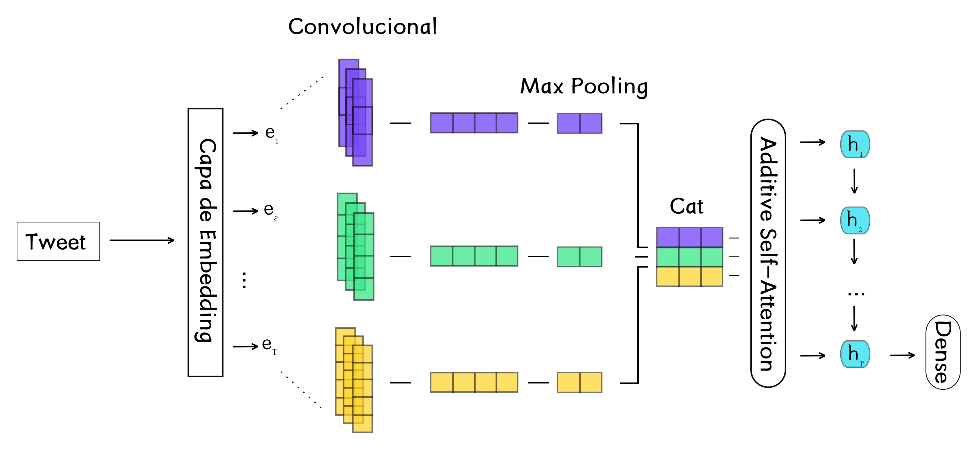
\includegraphics[]{images/cnn_lstm.eps}
		\end{center}	
		\caption[CNN - LSTM]{Arquitectura de Encoder CNN-LSTM}
		\label{cnn_lstm}
	\end{figure}
	\\
	Cada elemento de la secuencia es codificado por un \textit{embedding} de palabras o caracteres según sea el caso del análisis. En el primero, el modelo emplea un embedding preentrenado con representaciones fijas aprendidas mediante \textit{Word2Vec} de Google \citep{DBLP:conf/nips/MikolovSCCD13}. Mientras que a nivel de caracteres estas representaciones son inicializadas de manera aleatoria y aprendidas durante el proceso de entrenamiento del modelo completo.
	\\
	Como salida de esta capa de embedding obtenemos una matriz de valores reales $E \in \Re^{l\times d}$, con $l$ la longitud de la secuencia y  $d$ la dimensionalidad de la representación vectorial de sus elementos. Luego es aplicada la operación convolución en $1D$ mediante una capa de red convolucional, simulando el análisis de \textit{n-gramas} de palabras o caracteres sobre la representación del embedding que en este punto ya ha capturado ciertas relaciones de contexto entre los elementos del texto.
	\\
	Esta capa convolucional estará compuesta por filtros de distintos tamaños de ventana (3, 4, 5) inspirada en las Redes de Entradas (\textit{Inception Neural Networks}) \citep{szegedy2014going} para capturar relaciones espaciales dentro de la secuencia a corto plazo. Para cada tamaño de ventada (i.e., 3, 4 y 5) se emplean además 32 filtros que aprenden estas relaciones de manera independiente. 
	\\
	Una vez efectuada la convolución, sea $k$ el tamaño de la ventana, la longitud de la secuencia queda reducida a $l-k + 1$, luego para cada $k$ es aplicada la operación de \textit{max-pooling}, mediante la cual el modelo aprenderá a preservar solamente la información más relevante dentro de un \textit{n-grama}. El pooling se realiza de manera que en el paso $i-esimo$ la ventana no contempla los datos analizados en el paso $(i-1) -esimo$ por lo que el salto es equivalente al tamaño de la ventana, reduciendo nuevamente la secuencia a $\lceil\frac{l - k + 1}{k}\rceil$.
	\\
	La concatenación resultante de la\textit{ Inception Network} es considerada como una nueva secuencia de mapeo de rasgos, sin embargo, cada uno sus elementos se relacionan entre si aportando información relevante o no sobre la tarea a la cual responde el entrenamiento del modelo. Esta secuencia es procesada por una capa de \textit{self-attention} \textcolor{darkblue}{(Sección~\ref{atencion})} para ponderar los features teniendo en cuenta su nivel de importancia en vez de hacer a la red neuronal prestar atención de la misma forma a todos los elementos.
	\\
	Una vez combinada la información a través del mecanismo de atención, la secuencia es explorada y condensada por una LSTM, en la cual el fenómeno de \textit{information vanishing} estará inhibido gracias al mecanismo de atención. De la salida de la LSTM es preservado solamente el último estado oculto en el cual quedan capturadas relaciones a largo plazo en del estilo del autor y contenido del texto, finalmente es transformado a un elemento de un espacio latente por medio de una capa densa. Esta transformación constituye la representación del tweet con el que fue alimentado el modelo. 
	
	\subsection{Codificación basada en Transformers}\label{ref_trans}
	
	Teniendo en cuenta que al analizar individualmente los tweets la cantidad de información a procesar es reducida considerablemente y la capacidad de ``comprensión'' del lenguaje que han demostrado los modelos basados en arquitecturas Transformers (TM), se propone el empleo de modelos pre-entrenados para modelar representaciones abstractas de los tweets. Para ello primeramente se realiza un proceso de refinado (\textit{fine-tuning}) empleando la librería HuggingFace Transformers\footnote{\url{https://huggingface.co/transformers}} con datos que respondan a la tarea sobre la cual se llevará a cabo el perfilado. 
	\\\\
	En el proceso de \textit{fine-tuning} se añade una capa intermedia que recibe los vectores de la secuancia de salida del TM. En esta secuencia de features, se preserva solamente el vector asociado al \textit{token} [CLS]. Luego esta capa intermedia se apila una capa de salida encargada de realizar las predicciones para la tarea sobre la cual  se refina el modelo.
	\\
	Para cada uno de los bloques codificadores del encoder del Transformer es empleado un coeficiente de aprendizaje \textit{learning rate} distinto teniendo en cuenta un refinado gradual-discriminativo de cada bloque, incrementándolo a medida que la red se vuelve mas profunda. Esto es, $\alpha_i = \lambda_i \alpha_0 \text{ y } \lambda_i = \lambda_{i-1} + 0\text{.}1$, donde $\alpha_i$ representa el \textit{learning rate} del $i-esima$ bloque y $\lambda_i$ es un multiplicador para determinar $\alpha_i$ a partir de $\alpha_0$. Empleando este \textit{learning rate} dinámico se preserva la mayor cantidad de informacion aprendida durante el proceso de pre-entrenado el las capas más superficiales, encargadas de capturar rasgos generales, y se sesga el aprendizaje de las capas más profundas hacia la tarea específica abordada en el perfilado.
	\section{Modelado  y Clasificación del Perfil}
	
	Una vez sintetizada la información abstracta de los tweets, es importante la forma en la que se relaciona cada uno para clasificar el perfil, para ello se propone asumir el conjunto de los tweets como i) una secuencia y ii) una estructura basada en grafos.
	
	\subsection{Modelado Secuencial. Att-LSTM}\label{att-lstm}
	
	Aun cuando no existe necesariamente una relación temporal que exprese particularidades del estilo de escritura del perfil, es posible agregar la información de los tweets mediante una LSTM. Para ello, en el proceso de entrenamiento se construye una secuencia con los tweets, y en cada ciclo de entrenamiento (i.e., \textit{epoch}) de la red neuronal, esta secuencia es permutada aleatoriamente para evitar que el modelo capture erroneamente cualquier relación temporal. La \figurename~\ref{att_lstm} muestra la arquitectura general del modelo \textbf{Att-LSTM} (\textit{Attention- Long Short Term Memory}) empleada para modelar como secuencia el perfil y clasificarlo.
	
	\begin{figure}[!thb]
		\begin{center}
			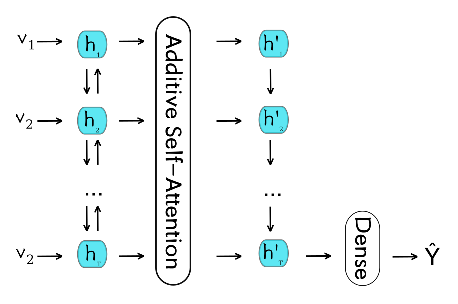
\includegraphics[]{images/att_lstm.eps}
		\end{center}	
		\caption[Att - LSTM]{Modelado y Clasificación del Perfil. Att-LSTM}
		\label{att_lstm}
	\end{figure}
	
	El modelo recibe una secuencia donde cada elemento corresponde a los rasgos extraídos para un tweet del perfil, esta secuencia es enviada a una LSTM Bidireccional (Bi-LSTM) \citep{DBLP:journals/tsp/SchusterP97}, la cual consiste en una célula de LSTM de 64 unidades que calcula para cada elemento dos estados ocultos concatenados, uno de ellos correspondiente a un recorrido de izquierda a derecha y el otro en sentido contrario.
	\\
	La Bi-LSTM no detecta solamente relaciones de un elemento con los previos en la secuencia sino que también lo relaciona con los que aparecen posteriormente, de esta forma se capturan las relaciones independientes de la posición de cada tweet dentro de la secuencia.
	\\ 
	La salida de la Bi-LSTM es enviada a una capa de \textit{self-attention} para emplear la misma estrategia propuesta en la \textcolor{darkblue}{Sección~\ref{cnn-lstm}} y luego a una capa de LSTM simple, donde nuevamente se preserva el último estado oculto y se condensa su información en una capa densa. Este modelado el perfil, finalmente es enviado otra capa densa encargada de clasificar el perfil según la tarea para la que se entrene el modelo.
	
	\subsection{Modelado basado en Grafo. SGN}\label{sgn}
	
	Dentro de las redes sociales en muchas ocasiones la información contextual es compartida de manera dispersa, e.g., el contenido de una idea relacionada con la difusión de odio puede ser construido relacionando la información de diferentes posts no necesariamente subidos de manera secuencial. Algunos trabajos han mostrado la importancia del contenido en tareas de AP \citep{OrtegaMendoza2018EmphasizingPI}, afirmando que rasgos basados en contenido a veces son más discriminativos que rasgos de estilo \citep{reddy2016survey}. Todo esto sugiere la idea de emplear una modelación no euclidiana del conjunto de tweets codificados y compartir la información de un tweets a los otros mientras que su información individual es transformada para expresar como este pertenece a su contexto.
	Las Redes Neuronales basadas en Grafo están especializadas en aprender patrones de este tipo de representaciones no estructuradas.
	\\
	El perfil es por tanto modelado con una representación basada en grafos, donde cada nodo es un tweet y cada uno de ellos esta conectado con todos los otros. Luego, este grafo es procesado por una Red Neuronal Convolucional Espectral en Grafos (\textit{Spectral Graph Convolutional Neural Network SGN}).
	\\
	El hecho de que cada nodo en el grafo modelado este conectado a todos los otros, hace que luego de un ciclo de paso de mensajes, un nodo individual, tenga conocimiento sobre cada nodo en el grafo, empleando el operador convolucional propuesto en \citep{kipf2017semisupervised} definido como:
	
	\begin{align}\label{matrix-wise}
		X' = ReLU(\hat{D}^{-\frac{1}{2}}\hat{A}\hat{D}^{-\frac{1}{2}}X\Theta)
	\end{align}
	
	Donde $X$ es la matris de representaciones vectoriales de los nodos, $\hat{A} = A + I$ es la matriz de adyacencia $A$ agregada a la matriz identidad $I$ lo que implica que autoconexiones para cada nodo son introducidas a la representación para que en el proceso de agregación se preserve su información original. La matriz $D$ es una matriz diagonal que contiene el grado del nodo $i-esimo$, i.e., $D_{ii} = |V|$ con $V$ el conjunto de los vértices. Finalmente, $\Theta$ es la matriz de parámetros de aprendizaje para determinar la codificación de cada nodo con sus rasgos que junto a la Matriz Laplaciana Normalizada expresan el nivel de variación entre los rasgos de los nodos dentro del grafo.
	\\
	Dada la formulación matricial de esta operación, a nivel de nodo esta queda definida como: 
	
	 \begin{align}\label{node-wise}
	 	x_i' = ReLU\left( \Theta \sum_{j \in \mathcal{N}(i) \cup \{i\}} \frac{1}{ 	\sqrt{ \hat{d_j} \hat{d_i} } }x_j \right)
	 \end{align}
	 \\
	 Aquí, $x_i$ representa la codificación del nodo $i-esimo$, $d_i$ el grado del mismo y $\mathcal{N}(i)$ su conjunto de nodos vecinos.
	 \\ 
	 Como es posible observar en \ref{node-wise} y \ref{matrix-wise}, en este esquema convolucional la información es compartida simplemente mediante una suma normalizada antes de calcular la nueva codificación $x_i'$ mediante $\Theta$.
	 \\
	 En la red convolucional propuesta este proceso de paso de mensaje y actualización es repetido a través de dos capas convolucionales. Luego, la información de los nodos es combinada a través de una capa de $mean-pool$ para alimentar una capa densa que sintetice la información. La salida de esta última capa es considerada como la modelación del perfil y es enviada a otra capa densa para realizar la clasificación.
	 
	 \section{Clasificación basada en ML. Deep Impostor }
	 
	 Un hecho interesante de sobre los modelos de DL es que a pesar de ser potentes a la hora de detectar rasgos abstractos que permitan particionar el espacio de representaciones en diferentes clases, cuando la cantidad de datos disponibles para el entrenamiento no es suficiente, su desempeño se ve afectado. Por esto se propone emplear las modelaciones  en un espacio latente de los perfiles descritas en la Sección~\ref{att-lstm} y Sección~\ref{sgn} con el Método Profundo de los Impostores \textit{(Deep Impostor Method DIM)} basado en el Método de los Impostores \citep{seidman2013authorship}, para realizar un estudio comparativo del desempeño en la clasificación binaria.
	 \\\\
	 Como en el método original, para realizar una predicción sobre un objeto desconocido (en este caso un perfil de autor) es definido previamente un conjunto $H$ y $K$ de ejemplos positivos y negativos respectivamente y el objeto desconocido $u$.
	 \\
	 De $H$ es muestreado de manera uniforme un subconjunto $\bar{H}$ como prototipos de la clase positiva y es analizado para cada $\bar{H}_i$ si $u$ es mas similar a este prototipo que a los elementos de un conjunto $\bar{K}_i$, i.e., $\mathcal{F}(u, \bar{H}_i) > \mathcal{F}(u, \bar{K}_{ij})$ donde $\mathcal{F}$ es una función de similitud; en este caso coseno. Luego de esto, se dice que $u$ teniendo en cuenta $\bar{H}_i$ es un candidato a pertenecer a una clase positiva según un voto por mayoría, esto es:
	 
	\begin{equation*}
	 	P_i(u,  \bar{H}_i) = 
	 	\begin{cases}
	 		1 & \text{if}~~ \sum\limits_{j}^{|\bar{K}_{i}|}[\mathcal{F}(u, \bar{H}_i) > \mathcal{F}(u, \bar{K}_{ij})] > \frac{|\bar{K}_{i}|}{2}\\
	 		0 & e.c.o.c
	 	\end{cases}
	 \end{equation*}	  
	 \\
	 Como los rasgos de los objetos serán aprendidos por medio de los modelos de DL descritos, es obviado el procedimiento de selección de rasgos expuesta en el método original, debido a que remover de manera indiscriminada alguno de ellos puede resultar en la destrucción de relaciones de similitud interclase o intraclase.
	 \\
	 Luego de definido cada $P_i$, un perfil $u$ es clasificado según la regla:
	 
	\begin{equation*}
	 	\hat{y}(u)  = 
	 	\begin{cases}
	 		1 & \text{if}~~ \sum\limits_{i}^{|\bar{H}|} P_i(u, \bar{H}_i) > \frac{|\bar{H}|}{2}\\
	 		0 & \text{otherwise}
	 	\end{cases}
	 \end{equation*}	
	 
	 
	 \section{Rasgos Manuales de Estilo}
	 
	 Para la representación del perfil es analizado un conjunto de 177 rasgos que capturen características relevantes del estilo de escritura. Los rasgos son estructurados en seis subconjuntos considerando diferentes capas textuales. Las capas son: booleanas; caracteres; oraciones; párrafo; sintáctica y de documento.
	 \\
	 Ejemplos de los elementos de estas capas son:	 \\
	 \begin{enumerate}
	 	\item Capa booleana: Usos de la misma palabra para terminar una oración y comenzar la siguiente.
	 	\item Capa de caracter: Media de la longitud de las palabras.
	 	\item Capa de oración: Media de la cantidad de palabras. Media de la cantidad de preposiciones distintas.
	 	\item Capa de párrafo: Media de la cantidad de oraciones. Media de la cantidad de palabras.
	 	\item Capa sintáctica: Proporción de sustantivos y adjetivos.
	 	\item Capa de documento: Media de la longitud de las oraciones.
	 \end{enumerate}
	 Esta representación es completamente independiente del genero textual e involucra valores con distintas estructuras de datos como se muestra en la \figurename~\ref{trepre}.

	 \begin{figure}[!thb]
	 	\centering
 	 	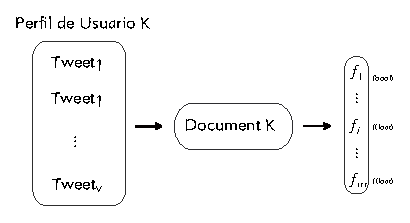
\includegraphics[width=.65\linewidth, , height=.2\textheight]{images/trepre.eps}
	 	\caption[Rasgos Manuales]{Representación de perfil mediante rasgos manuales}
	 	\label{trepre}
	 \end{figure}
	 
	 
	 
	\chapter{Marco Experimental}

En este capítulo, son descritos los conjuntos de datos sobre los que se evaluará el desempeño de la estrategia de análisis modular propuesta para abordar el perfilado de autores. Luego se exponen las metricas empleadas y finalmente se presentan los resultados experimentales asociados a cada módulo (i.e., Codificador y Clasificador) de manera independiente y a las combinaciones de los mismos.
	
\section{Tareas}
	 
	 Las colecciones de datos existente relacionadas con tareas de AP mayormente se encuentran anotadas a nivel de perfil y con información relativa a tareas especificas. Para evaluar los modelos propuestos, siguiendo este esquema, en este trabajo se introducen los conjuntos de datos de las tareas compartidas en las ediciones de 2019-2021 de PAN, cada una de estas propuestas con un enfoque multilingüe, analizando el problema para perfiles de usuarios del idioma ingles y español.
	 
	 \subsection{Bots and Gender Profiling at PAN 2019}
	 
	 En la tarea Bots and Gender Profiling, dado conjunto de exactamente 100 posts  pertenecientes a un perfil de usuario de Twitter y teniendo en cuenta que no existe ningún tipo anotación a nivel de tweets, debe determinarse si este corresponde a un bot o a un ser humano y para el segundo caso predecirse el genero sexual de la persona.
	 \\
	 Para evaluar el desempeño de los modelos propuestos, en nuestro trabajo se prestará atención solamente al problema de discernir entre perfiles de usuarios humano hombres o mujeres. El conjunto de datos de perfiles humanos está construido a partir de cuentas de usuarios tomadas de corpus creados en ediciones previas de la tarea de perfilado de PAN \citep{rangel2017overview, rangel2018overview}. Además los datos se encuentran distribuidos uniformemente tanto para el idioma ingles como para el español, entre las clases `\textit{Male}' y `\textit{Female}' como puede ser observado en la \tablename~\ref{pan19data}.	 
	 		\begin{table}[thb!]
			 	\begin{center} 					 		
			 		\begin{tabular}{lcccccc} 
			 			\specialrule{.1em}{.05em}{.05em}
			 			 \multirow{2}{*}{}&\multicolumn{3}{c}{(EN) Ingles}&\multicolumn{3}{c}{(ES) Español}\\	 			\cline{2-7}
			 			&~~Female~~&~~Male~~&~~Total~~ &~~Female~~ &~~Male~~&~~Total~~\\
			 			\specialrule{.1em}{.05em}{.05em} 
			 			Training & 1030&1030&2060&750&750&1500\\
			 			Test  &660&660&1320&450&450&900\\
			 			\cline{1-7}
			 			Total &1690&1690&3380&1200&1200&2400\\
			 			\specialrule{.1em}{.05em}{.05em} 
			 		\end{tabular}
			 		\label{pan19data}	
			 		\caption[Corpus Profiling PAN 2019]{Distribución de los datos para la tarea Bots and Gender Profiling at PAN 2019}	
			 	\end{center}
			 \end{table}	
		 \\
	 \subsection{Profiling Fake News Spreaders on Twitter at PAN 2020}
	 
	 Profiling Fake News Spreaders on Twitter, dentro de PAN 2020, introduce el análisis de rasgos de la personalidad de los autores, proponiendo la tarea de discriminar entre usuarios de Twitter que han compartido noticias falsas de aquellos que nunca lo han hecho, basándose en un conjunto de 100 tweets (carentes de algún tipo de anotación) tomados de su perfil.\\
	 El corpus propuesto por los organizadores de la tarea \citep{francisco_rangel_2020_4039435}, fue construido seleccionando de sitios web  \textit{fact-checking } (comprobadores de hechos) noticias etiquetadas como falsas, luego mediante la búsqueda de tweets relacionados con estas \textit{fake news}, se identificaron a sus correspondientes usuarios como ejemplos positivos de \textit{fake news spreaders} (faker) tomando aquellos con un mayor número de noticias falsas compartidas y teniendo en cuenta que el contenido del tweet no fuera para desmentir la noticia falsa.	 En el caso de que el usuario no hubiera compartido información relacionada con las noticias falsas identificadas, este fue etiquetado como \textit{real news spreader} (no faker).
	 
	 El la \tablename~\ref{pan20data} se muestra la distribución uniforme de los perfiles para los idiomas español e ingles en los que fue compartida la tarea.	 
	 
	 	\begin{table}[thb!]
	 	\begin{center} 					 		
	 		\begin{tabular}{lcccccc} 
	 			\specialrule{.1em}{.05em}{.05em}
	 			\multirow{2}{*}{}&\multicolumn{3}{c}{(EN) Ingles}&\multicolumn{3}{c}{(ES) Español}\\	 			\cline{2-7}
	 			&~~faker~~&~~no faker~~&~~Total~~ &~~faker~~ &~~no faker~~&~~Total~~\\
	 			\specialrule{.1em}{.05em}{.05em} 
	 			Training & 150&150&300&150&150&300\\
	 			Test  &100&100&200&100&100&200\\
	 			\cline{1-7}
	 			Total &250&250&500&250&250&500\\
	 			\specialrule{.1em}{.05em}{.05em} 
	 		\end{tabular}
	 		\label{pan20data}	
	 		\caption[Corpus Profiling PAN 2020]{Distribución de los datos para la tarea Profiling Fake News Spreaders on Twitter at PAN 2020}	
	 	\end{center}
	 \end{table}	
	 
	 \subsection{Profiling Hate Speech Spreaders on Twitter at PAN 2021}
	 
	 Para esta tarea dado un perfil de usuario, debía ser determinado cuando este corresponde a un autor que ha difundido en el pasado un discurso de odio teniendo en cuenta 200 tweets tomados de su perfil.\\
	 El corpus propuesto por los organizadores fue construido considerando usuarios que han empleado palabras con cierto nivel de toxicidad fundamentalmente relacionadas con la misoginia y xenofobia, ademas se inspeccionaron cuentas de usuarios conocidos como \textit{haters} con apariciones en reportes, asi como su red i.e., followers. Luego para estos usuarios identificados, fueron anotados manualmente los tweets que comunicaban un discurso de odio y finalmente fueron clasificados como \textit{hate speech spreaders} aquellos usuarios con mas de 10 de estos posts. El conjunto de datos esta distribuido uniformemente para las clases divulgador de discurso de odio (\textit{hater})  y no divulgador de discurso de odio (\textit{no hater}) como se muestra en la \tablename~\ref{pan21data}
	 
	 
	 	\begin{table}[thb!]
		 	\begin{center} 					 		
		 		\begin{tabular}{lcccccc} 
		 			\specialrule{.1em}{.05em}{.05em}
		 			\multirow{2}{*}{}&\multicolumn{3}{c}{(EN) Ingles}&\multicolumn{3}{c}{(ES) Español}\\	 			\cline{2-7}
		 			&~~hater~~&~~no hater~~&~~Total~~ &~~hater~~ &~~no hater~~&~~Total~~\\
		 			\specialrule{.1em}{.05em}{.05em} 
		 			Training & 150&150&300&150&150&300\\
		 			Test  &100&100&200&100&100&200\\
		 			\cline{1-7}
		 			Total &250&250&500&250&250&500\\
		 			\specialrule{.1em}{.05em}{.05em} 
		 		\end{tabular}
		 		\label{pan21data}	
		 		\caption[Corpus Profiling PAN 2021]{Distribución de los datos para la tarea Profiling Hate Speech Spreaders on Twitter at PAN 2021}	
		 	\end{center}
		 \end{table}	
	 
	 \section{Resultados Experimentales}
	 
	 La robustez de los sistemas modulares descansan en el optimo aprendizaje de cada uno de los módulos de manera independiente, en nuestro caso del Codificador y el Clasificador. De manera general en nuestro trabajo introducimos una tarea intermedia semisupervisada para entrenar los modelos Codificadores \footnote{El objeto de predicción de esta tarea semisupervisada, estuvo condicionado por la carencia de anotación a nivel de tweet en cada uno de los corpus y se relaciona con la pertenencia o no a determinado tipo de perfil.}, de esta forma los mismos aprenden relaciones del lenguaje dentro de cada tweet sobre la tarea en cuestión.\\
	 Para medir el cuan efectivos resulta cada modelo empleamos las métricas \textit{accuracy} (\ref{accuracy}) y\textit{ recall} (\ref{recall}), esta última para los modelos de clasificación sobre la clase positiva en las tareas en las que es necesario la correcta identificacion de una clase sobre otra, i.e., clase positiva (hater) en \textit{Profiling Hate Speech Spreaders on Twitter}  y clase positiva (faker) en \textit{Profiling Fake News Spreaders on Twitter}.
	 
	 \begin{flalign}
	 	acc=~& \frac{TP + TN}{TP + FP + TN + FN}\label{accuracy}\\
	 	recall =~& \frac{TP}{TP + FN}\label{recall}
	 \end{flalign}
 
 	\subsection{Codificador CNN - LSTM}
 	\subsection{Codificador Transformer}
	\bibliographystyle{style/acl_natbib}
	\renewcommand{\bibname}{Referencias Bibliográficas}
	\bibliography{bibliography}
	
\end{document}